\documentclass[crop,tikz]{standalone}

\begin{document}
  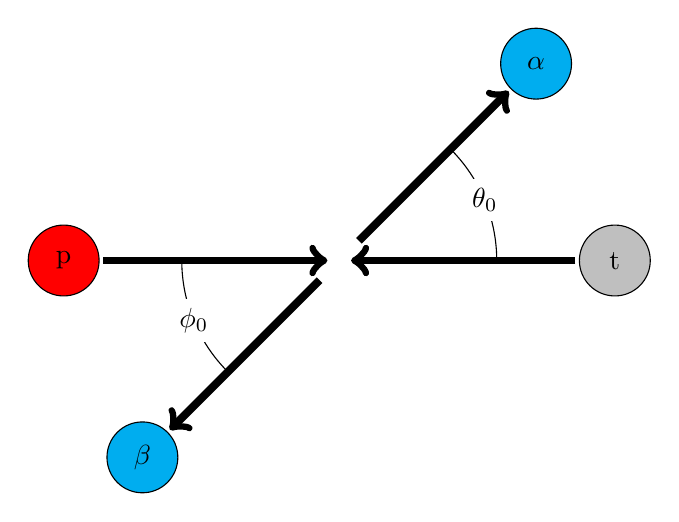
\begin{tikzpicture}
    \node[circle, draw, fill=red,       minimum size = 0.9cm] (c) at (-3.5,0){p}; 
    \node[circle, draw, fill=lightgray, minimum size = 0.9cm] (c) at ( 3.5,0){t}; 
    \draw [-to, line width=1mm] (-3,0) -- (-0.15,0);
    \draw [-to, line width=1mm] ( 3,0) -- ( 0.15,0);
    \node[circle, draw, fill=cyan, minimum size = 0.9cm] (c) at ( 2.5,  2.5){$\alpha$};
    \node[circle, draw, fill=cyan, minimum size = 0.9cm] (c) at (-2.5, -2.5){$\beta$};
    \draw [-to, line width=1mm] ( 0.25, 0.25) -- ( 2.15, 2.15);
    \draw [-to, line width=1mm] (-0.25,-0.25) -- (-2.15,-2.15);
    \draw ( 2,0) arc [start angle=0,   end angle=45,  x radius=2cm, y radius =2cm] node[midway,fill=white] {$\theta_0$};
    \draw (-2,0) arc [start angle=180, end angle=225, x radius=2cm, y radius =2cm] node[midway,fill=white] {$\phi_0$};
  \end{tikzpicture}
\end{document}